\scanpage{62}

d'ordre \inserted{$d'$} divisant $d$, et a fortiori $d^t$.
\figure{
\begin{tikzpicture}[x=.6cm,y=.6cm,line cap=round]
\draw[line width=.35pt] (.12,.95)..controls (-.18,1.12) and (-.23,.22)..(.34,.22)..controls (.62,.22) and (.73,.04)..(.76,-.18);
\draw[line width=.55pt] (.76,-.18)..controls (.84,.23) and (1.29,.58)..(1.36,.94);
\end{tikzpicture}}

c) \deleted{Pour tout} Soit $n$ un entier, et supposons que $n$ est premier à $p$, \uline{ou} que \inserted{$d_t$ est premier à $p$, o\unsure{ú|ù} que} $k$ est p\unsure{\deleted{r}a}\unsure{\deleted{a}r}fait(donc algébriquement clos).On a alors une suite exacte canonique, fonctorielle en $X$:
\figure{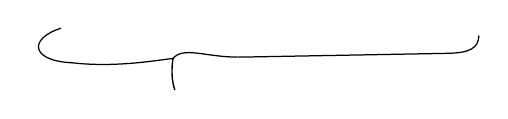
\begin{tikzpicture}[x=.75cm,y=.6cm,line cap=round]
\draw[line width=.45pt] (.35,.65)..controls (-.2,.43) and (-.16,-.04)..(.54,-.08)..controls (1.32,-.19) and (2.04,-.01)..(2.25,.01)..controls (2.43,.28) and (2.8,.03)..(3.4,.04)--(6.9,.12)..controls (7.28,.13) and (7.42,.23)..(7.43,.49);
\draw[line width=.5pt] (2.25,.01)..controls (2.22,-.24) and (2.23,-.46)..(2.28,-.65);
\end{tikzpicture}}
\diagram{\begin{tikzcd}[ampersand replacement=\&,column sep=small]
(6)\quad 0\arrow[r]\&{}_n\Gamma\arrow[r]\arrow[d,phantom,"{\rotatebox{90}{$\simeq$}}" description]\&H^1(X,\mu_n)\arrow[r,"u_n"]\&H^1(X_{\bar\eta},\mu_n)^I\arrow[r]\&\operatorname{Ker}\deleted{{}_{\unsure{n}}}w_n\arrow[r]\&0,\\
\&\inserted{\mathbb Z/(n,d)\mathbb Z}\&\&\&\&
\end{tikzcd}}
où
\[
w_n:\Gamma_n\longrightarrow\operatorname{NS}(X_{\unsure{0|o}})_n
\]
est l'homomorphisme déduit de (5) pa\unsure{\deleted{d}r} tensorisation par $\underline Z/n\underline Z$, \deleted{\unsure{Pour} $n$ variable \unsure{multiplic|multiplier}} et où $u_n$ est l'homomorphisme canonique (\qquad).

Pour $n$ variable multiplicativement, les suites exactes (6) forment un système projectif de suites exactes, p\deleted{a}\inserted{o}ur les morphismes de transition évidents.

\margin{\figure{\begin{tikzpicture}[x=.55cm,y=.55cm,line cap=round]
\draw[line width=.35pt] (0,2.45)--(.16,2.88);\draw[line width=.3pt] (.04,2.69)--(.18,2.43);
\draw[line width=.3pt] (.12,1.32)--(.34,1.7);\draw[line width=.45pt] (.09,1.52)--(.39,1.27);
\draw[line width=.25pt] (.26,.02)--(.57,.5);\draw[line width=.4pt] (.27,.24)--(.59,.06);
\end{tikzpicture}}}

d) Soit $\ell$ un nombre premier, \deleted{et supposons $\ell\neq p$ ou $k$ parfait\unsure{.}}\deleted{\inserted{ou $d_t$ premier à $p$ ou}}
\figure{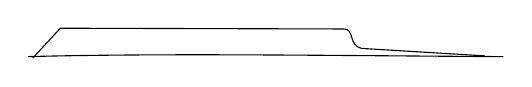
\begin{tikzpicture}[x=.27pt,y=-.27pt]
\draw (6,40)--(43,0)--(422,1)..controls (437,0) and (428,23)..(446,27)--(611,37);
\draw (0,38)..controls (186,33) and (436,37)..(636,38);
\end{tikzpicture}}
 Alors on \deleted{trouve}\inserted{a} une suite exacte canonique, \inserted{fonctorielle en $X$} \deleted{(obtenue, si $\ell$ satisfait \inserted{aux \unsure{conditions} de c)}, par passage à la limite projective sur les puissances de $\ell$ dans les suites exactes (6)):}\deleted{on \unsure{trouvera|trouve} une suite exacte}
\figure{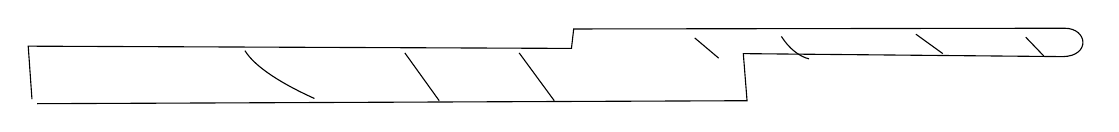
\begin{tikzpicture}[x=.27pt,y=-.27pt]
\draw (5,95)--(0,24)--(727,27)--(730,1)--(1387,0)..controls (1418,0) and (1422,37)..(1385,38)--(957,34)--(962,97)--(12,101);
\draw (290,30)..controls (304,53) and (343,76)..(383,94);
\draw (504,33)--(550,97);
\draw (657,33)--(704,97);
\draw (892,13)--(924,40);
\draw (1008,11)..controls (1018,27) and (1032,38)..(1045,41);
\draw (1188,8)--(1224,34);
\draw (1335,12)--(1359,37);
\end{tikzpicture}}
\diagram{\begin{tikzcd}[ampersand replacement=\&,column sep=small]
(7)\quad0\arrow[r,phantom,"{\unsure{\longrightarrow|\mathbin{-}}}" description]\&H^1(X,\underline Z_\ell(1))\arrow[r,"u(\ell)"]\&\rlap{\raisebox{-.85ex}{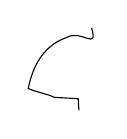
\begin{tikzpicture}[x=.45cm,y=.45cm,line cap=round]
\draw[line width=.4pt] (1.65,1.5)..controls (1.84,.85) and (1.35,1.48)..(.95,1.24)..controls (.45,1.07) and (.03,.65)..(-.14,-.2)..controls (.07,-.3) and (.36,-.34)..(.6,-.45)--(1.27,-.49)--(1.29,-.81);
\end{tikzpicture}}}H^1(X_{\bar\eta},\underline Z_\ell(1))^I\arrow[r]\&R\otimes\underline Z_\ell\arrow[r]\&0,
\end{tikzcd}}
où $R=\operatorname{Ker}w\simeq\underline Z/d'\underline Z$, donc
\[
\rlap{\raisebox{-.1ex}{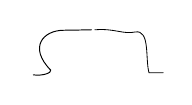
\begin{tikzpicture}[x=.55cm,y=.55cm,line cap=round]
\draw[line width=.35pt] (-.38,.05)..controls (-.16,.02) and (.05,.1)..(.02,.16)..controls (-.5,.69) and (-.15,1.08)..(.32,1.08)--(.96,1.09);
\draw[line width=.3pt] (1.04,1.09)..controls (1.49,1.13) and (1.69,.98)..(1.97,1.04)..controls (2.32,1.1) and (2.2,.43)..(2.29,.1)--(2.62,.1);
\end{tikzpicture}}}(8)\qquad R\otimes\underline Z_\ell\simeq
\begin{cases}
0\text{ si }\ell\unsure{\deleted{\neq}\inserted{\nmid}}d',\quad\inserted{\text{a fortiori si }\ell\nmid d^t,}\\
\underline Z/\ell\underline Z\text{ si }\ell\mid d'.
\end{cases}
\]
\margin{\figure{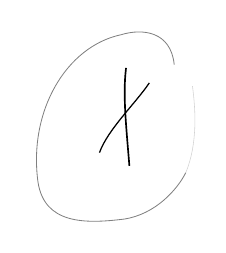
\begin{tikzpicture}[x=.6pt,y=-.6pt]
\draw[gray,line width=.3pt] (88,22)..controls (86,2) and (69,0)..(56,4)..controls (23,11) and (0,50)..(6,93)..controls (10,118) and (34,118)..(58,115)..controls (77,112) and (90,97)..(95,87);
\draw[gray!35,line width=.2pt] (95,87)..controls (102,70) and (101,50)..(99,35);
\draw[line width=.6pt] (59,24)..controls (57,40) and (59,58)..(61,83);
\draw[line width=.45pt] (43,75)..controls (48,61) and (65,45)..(73,33);
\end{tikzpicture}}}

On obtient en particulier\unsure{*}, grâce à d)\inserted{:} {\setbox0=\hbox{\let\ScanOverlaySavedSout\sout\let\sout\relax\deleted{\let\sout\ScanOverlaySavedSout\unsure{du|au} moins si $\ell\neq p$:}}
\dimen0=\wd0
\dimen2=\ht0\advance\dimen2 by \dp0\advance\dimen2 by 4pt
\leavevmode\rlap{\raisebox{\dimexpr-\dp0-2pt\relax}{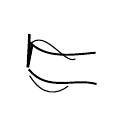
\begin{tikzpicture}[x={\dimexpr\dimen0/377\relax},y={\dimexpr-\dimen2/33\relax}]
\path[use as bounding box] (0,0) rectangle (377,33);
\draw[line width=.7pt] (372,12)..controls (245,13) and (99,15)..(12,7)--(0,19);
\draw[line width=.7pt] (377,27)..controls (256,24) and (107,31)..(6,20);
\draw (13,8)..controls (95,0) and (203,18)..(261,15);
\draw (11,23)..controls (80,33) and (163,32)..(222,28);
\draw[line width=.9pt] (1,19)--(10,3) (1,19)--(25,8);
\end{tikzpicture}}}\box0}

\uline{Corollaire} \inserted{9}. \deleted{L'homomorphisme} Soit $\ell$ un nombre premier, \deleted{\unsure{tel que l'on ait $\ell\neq p$ si $k$ n'est pas parfait ou $d_t$}} Alors l'homomorphisme
\[
(\hspace{1em}\inserted{10})\qquad u(\ell):H^1(X,\underline Z_\ell(1))\longrightarrow H^1(X_{\bar\eta},\underline Z_\ell(1))^I
\]
est injectif, son conoyau est un groupe fini, nul pour presque tout $\ell$.
La même conclusion est vraie en remplaçant $\underline Z_\ell(1)$ par $\underline Z_\ell$, à co\unsure{\deleted{j}n}dition de supposer $\ell\neq p$.

\margin{\figure{\begin{tikzpicture}[x=.5cm,y=.5cm,line cap=round]
\draw[line width=.3pt] (0,0)--(.27,.45);\draw[line width=.45pt] (.04,.29)--(.38,.06);
\end{tikzpicture}}}
\margin{\figure{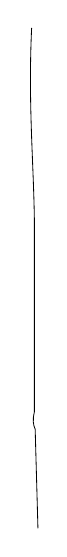
\begin{tikzpicture}[x=.5cm,y=.5cm,line cap=round]
\draw[line width=.3pt] (0,12.8)..controls (-.09,10.9) and (.05,9.4)..(.07,7.9)--(.07,3.05)..controls (.02,2.85) and (.04,2.72)..(.09,2.61)--(.16,.1);
\end{tikzpicture}}}
\margin{\figure{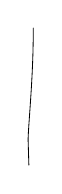
\begin{tikzpicture}[x=.5cm,y=.5cm,line cap=round]
\draw[line width=.3pt] (.19,3.55)..controls (.2,2.4) and (.07,1.15)..(.06,.72)--(.08,.07);
\end{tikzpicture}}}
\margin{61}
